\chapter{Design}
\section{Design Methods}
What methods have been used, what user experiences and usability goals have we found out?
%%%%%%%%%%%%%%%%%%%%%%%%%%%%%%%%%%%%%%%%%%%%%%
\subsection{Usability goals}\textit{Dennis.}\\
Different sessions have been done with the customer and based on that some usability goals and user experience goals have been set and given points due its priority. The sessions with the customer will 
The below sections will be given points on a scale from 1 to 10, depending on
the importance (were 10 is very important and 1 is less important)
\begin{itemize}
	\item 10 safe to use (safety)
	\item 8 easy to learn (learnability) 
	\item 8 easy to remember how to use (memorability)
	\item 6 effective to use (effectiveness) 
	\item 5 efficient to use (efficiency/performance)
	\item 3 have good utility (utility)	
\end{itemize}
\subsubsection{Safety}
Most important is the safety factor as the user of the system (Jan) should be able to show the system for high-school students and others without some fiddle-fingers is hurt. Therefore everything dangerous such as: high voltage connections and sharp edges should be held inside the module boxes.
Non-technically experienced persons should also be able to connect devices to the system, not thinking about safety risks. 
\subsubsection{Learnability}
As the system is meant to be operated by a non-technically person, learning the system should be fast and operating the system should therefore be very intuitive. 
Also visitors should be able to do simple tasks on the system, such as turn a device on or off.
\subsubsection{Memorability}
Mainly the system is supposed to run by it self without any interaction. But when the system is going to be operated on or the system is showed to some visitors, the instructed person(s) should be able to do so without any preparation time.
\subsubsection{Effectiveness}
The effectiveness of the system is not the most important factor, but still quiet important as we are talking about a green system, which should be
affordable for the user to implement. When investing in a green system, normally it will have some information about estimated lifetime and buy time (the time
it takes the system to `buy home itself'). If the buy time is to long, maybe longer than the lifetime, the price for having such a system will be way to high. 
Visitors should also be able to see the advantage in buying a green system (environmental and money friendly), so it might affect them to be more environmental friendly. 
\subsubsection{Efficiency/Performance}
The performance in the system is not critical when considering it from the users perspective. It doesn't matter if it takes a few seconds before the system responds the user. But for safety reasons it should be operate very fast between the modules so no parts is harmed due to too long response time.
\subsubsection{Utility}
The possibility of changed a lot of parameters in the system should be kept as low as possible to easy the interaction with the system. If the user has too many ways of setting up the system it can easily confuse more than necessary. Therefor only the most important things that the user should be able to change is implemented, rest of the settings should be placed as hidden utilities. 

%%%%%%%%%%%%%%%%%%%%%%%%%%%%%%%%%%%%%%%%%%%%%%
\subsection{User experience goals}\textit{Dennis.}\\
The user should not find this system specially emotional or fun as the system might be seen as frivolous if it is overdone. However, to keep the interest of the visitors (primarily high school students), the system should be entertaining to a certain level.  
Down below the different user experience goals are listed in order (so most important at the top):
\begin{enumerate}
	\item Rewarding
	\item Helpful
	\item Entertaining
	\item Motivating
	\item Enjoyable
	\item Fun
	\item Satisfying
	\item Aesthetically pleasing
	\item Emotionally fulfilling
\end{enumerate}


\begin{wrapfigure}{r}{0.4\textwidth}
	\center
		\setlength\fboxsep{0pt}
		\setlength\fboxrule{0pt}
		\fbox{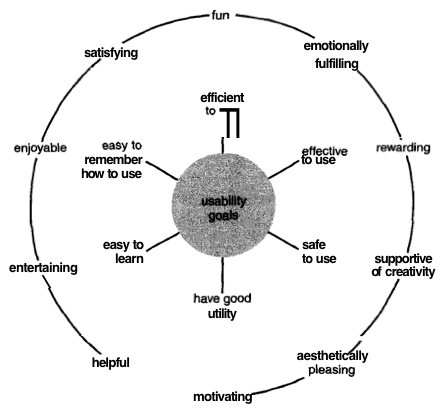
\includegraphics[width=0.4\textwidth]{images/usability_goals_diagram.png}}
   	\caption{\textit{The difference between usability and user experience goals, where  usability goals are central to
  			interaction design and are operationalized through specific criteria. 
  			User experience goals are shown in the outer circle and are less clearly defined.}}
   	\label{fig:index_page_design}
\end{wrapfigure}
\textbf{ }\\ \\ 
The goal is to give visitors a better understanding of the term 'Green Energy'. They should feel like they have become rewarded on the area after having interacted with the system. The system should be helpful, to easy the process of doing things, like seeing the production historic, connected modules etc. The values represented are represented as non-technically expressions to make it more entertaining and to not make the user lose motivation. Even though the user should learn something by using the system, the system is also supposed be enjoyable and fun to use. Emotionally fulfilling devices and aesthetically pleasuring is mostly consumer devices (PC's, cell-phones, TV etc.), where this device is not seen as a part of.
%%%%%%%%%%%%%%%%%%%%%%%%%%%%%%%%%%%%%%%%%%%%%%